\chapter{Consistency through different transcriptomics studies with RNA-Seq}
\label{ch:Transcriptomics}
\setlength{\epigraphwidth}{0.45\textwidth}
\setlength{\epigraphrule}{0.1pt}
\epigraph{Quantifier: c'est convenir, puis mesurer.}{\cite{Desrosieres}}


I started this project in January 2013. At that time, there was no
literature comparing normal human transcriptome tissues across different datasets.

\section{Introduction}

\begin{itemize}
    \item Difficulty of sampling of normal conditions for human, particularly
        for the solid tissues. (could be very useful in case of cancer for
        example)
    \item Lots of transcriptomics data in the repository of EBI. Can we use
        this as a base for reference? + Explosion of atlases publications
    \item previous point not new, but recently multiplications of studies on
        normal human studies based on \Rnaseq
    \item Indeed, in the past people tried with microarray data but didn't work
        \TK{find sources}
    \item When I started this study, there wasn't any publication on this matter
        yet, but \Rnaseq was considered as quantitative (when microarrays were
        considered semi-quantitative at best).
    \item nobody did published on my specific subject yet, but since then things changed
    \item first paper from MACQ/SEC III
    \item increasing number of papers that been published on the subject
    \item I will discuss the different part of the papers that are relevant
        with additions on what my study confirms/refutes or expands them.
\end{itemize}

Progress in Science is based on different elements. In natural sciences, notably
Biology, repeated observations are one of the earliest ones. Then quantifications
when possible (+ definitions give you characterisation). (They could be inferred or
been used as a start for a hypothesis and then there are predictions and
experiments). When many observations and measurements, common step: try to create
a reference. People tried with microarrays technologies but there were too many
biases and too different microarrays to work with. However, it would be very nice
to have a reference as it is hard to have a normal controls in studies. Hence, we
have seen a common trend of Atlases publications and even more when \Rnaseq\ started
to be used more commonly. (Explosion of the Atlases).

While current high-throughput gene expression studies are mainly about
differential gene expression between (notably diseased and treated) conditions,
healthy controls are not always enough or even available. Even more so, when the
study subject is human. Indeed, it rather apprehensible that sampling solid
tissues on a healthy human is not (and should not be) usual or common.

Although, many atlases have been released to help on this issue,
there is still not any direct method that would allow you more than check the
presence (or lack of detection) of specific genes in a given condition.

With the increasing number of studies of normal tissues with overlapping conditions
\cref{fig:VennStudiesT}, we are investigating the consistency of gene-tissue
associations on
one side but moreover we would like to assess the expression levels across the
datasets in the aim of integrating all the available data in a gene expression
baseline reference.

When I started this project there was not any study, comprehensive or not, that
was investigating in-depth the consistency of transcriptome expression measurements
for one condition across studies.


As previously stated in the introduction, while I started this project,
there wasn't any study that was investigating in-depth the reproducibility of
transcriptomics.

However, in August 2014 a paper comparing different preparation methods,
sequencing technologies operated in different laboratories
on samples from the same biological source concludes that while absolute
measurements are not consistent, the relative expression is highly consistent
(95\% Pearson correlation?)

The main question when I started this project was to appraise how much consistent
(robust) is the \Rnaseq technology to quantify the gene expression. While it
is comparable to microarrays for differential gene expression analysis study
\TK{add reference},
\Rnaseq\ plus: detect new things - minus: sampling problems (stuff might be there
but won't be ``fished''.


\section{Available studies}
\label{sec:Trans_AvailableStudies}

All the datasets with which I worked are fitting three main criteria.
They comprise human normal samples from at least three kind of tissues.
They have been sequenced with \Rnaseq\ and
the \emph{raw} data is available and reuseable.
While they are quite a few more studies that I would have like to use
this last point was often the critical reason why they have not been included.
Indeed, many times I encountered data with ambiguous encoding format and, as the
studies were a little bit outdated,
I also could not get the information from the original authors.

When I started this work in 2013, there were only three complying
datasets at that time. Fortunately, I was later
able to incorporate two other datasets to my study. One of them is the \Gtex\
pilot (version 1.4) data and the other one is the Uhlén et al.\ dataset (first
published as \citet{Uhlen2014} and then extended for the \citet{Uhlen2015} publication).
The number of provided samples and covered tissues for these two datasets
is far greater than the other ones. These \dataset{\Gtex} and \dataset{Uhlén}
datasets are indeed presenting a greater set of common tissues. Moreover,
the more recent and similar technology used (either for the libraries preparation,
the sequencer or the paired-end protocols) and the studies design that includes
biological replicates for every tissue had motivated a more focused comparison
based only on these two datasets.

While I downloaded and entirely processed four of the transcriptomic datasets
myself, it was not the case for the \Gtex\ dataset. Since this
data is involved in many project within the \EBI\ and due to its huge amount of
data, it was agreed that this would be processed centrally by one person and then
redistributed to all the other interested parties.

For the sake of consistency, that led me to reprocess all the other four datasets
to comply with the reference used for the \Gtex\ samples. The silver lining
was that they were built with the new reference of the
Human genome GRCH 38 (ENSEMBL v. 76).

\begin{figure}%[!htbp]
    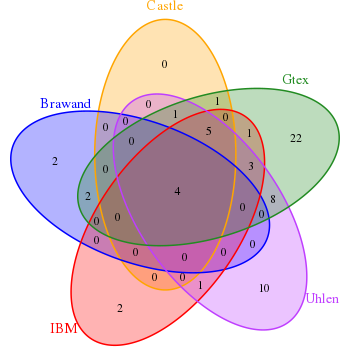
\includegraphics[scale=0.6]{transcriptomics/VennStudiesT}\centering
    \caption[Distribution of unique and shared tissues between the
    transcriptomic datasets]
    {\label{fig:VennStudiesT}\textbf{Distribution of unique and shared tissues
    between the transcriptomic datasets.} The 5 datasets share 4
    common tissues: \tissue{Heart}, \tissue{Kidney}, \tissue{Liver} and
    \tissue{Testis}. The biggest overlap of tissues (23) is between Uhlén et \Gtex.
    These two sets of tissues are the focus of the current study.}
\end{figure}

\Cref{fig:VennStudiesT} presents the five datasets overlapping tissues. We notice
that they all share at least four tissues: \tissue{Heart}, \tissue{Kidney},
\tissue{Liver} and \tissue{Testis}.

We also observe the great number of shared tissues between the two most recent
datasets: \dataset{Uhlen} and \dataset{GTEx}. Indeed, they share together twenty-three
tissues: \tissue{Adipose}, \tissue{Adrenal}, \tissue{Bladder},
\tissue{Cerebral cortex}, \tissue{Colon}, \tissue{Oesophagus},
\tissue{Fallopian tube}, \tissue{Heart}, \tissue{Kidney}, \tissue{Liver},
\tissue{Lung}, \tissue{Ovary}, \tissue{Pancreas}, \tissue{Prostate},
\tissue{Salivary gland}, \tissue{Skeletal muscle}, \tissue{Skin},
\tissue{Small intestine}, \tissue{Spleen}, \tissue{Stomach}, \tissue{Testis},
\tissue{Thyroid} and \tissue{Uterus}.

The \cref{tab:Trans5DF} summarises the main characteristics of the different
datasets. We can see that many of them have been produced through
polyA-selected library protocols. To avoid as many artefacts as possible, I
focus my study on the \mRNAs\ pool: most of the analyses are excluding
any gene that the biotype is not annotated as \emph{protein coding}.

I describe hereafter the datasets in the
chronological order of their first publication.

\begin{sidewaystable}
    \centering
    \caption{\label{tab:Trans5DF}Technical description of the 5 transcriptomic
    dataset (\Rnaseq)
     used for this study}
\begin{tabular}{@{}cccccccccc@{}}
\toprule
\multicolumn{1}{c|}
    {\multirow{2}{*}{ArrayExpress ID}} &
     \multicolumn{1}{c|}{\multirow{2}{*}{Data ID}} &
     \multicolumn{2}{c|}{\begin{tabular}[c]{@{}c@{}}Library\\Preparation\end{tabular}} &
     \multicolumn{2}{c|}{Sequencing} &
     \multicolumn{2}{c|}{Replicates} &
     \multicolumn{1}{c|}{\multirow{2}{*}{\begin{tabular}[c]{@{}c@{}}Tissue\\
             Number\end{tabular}}} &
     \multirow{2}{*}{\begin{tabular}[c]{@{}c@{}}Multi-sampling\\ from the \\ same individual\end{tabular}} \\
     \cmidrule(lr){3-8}
     \multicolumn{1}{c|}{} & \multicolumn{1}{c|}{} &
     \multicolumn{1}{c|}{\begin{tabular}[c]{@{}c@{}}Whole\\ RNA\end{tabular}} &
     \multicolumn{1}{c|}{\begin{tabular}[c]{@{}c@{}}PolyA\\ selected\end{tabular}} &
     \multicolumn{1}{c|}{\begin{tabular}[c]{@{}c@{}}Single\\ end\end{tabular}} &
     \multicolumn{1}{c|}{\begin{tabular}[c]{@{}c@{}}Paired\\ end\end{tabular}} &
     \multicolumn{1}{c|}{Biological} & \multicolumn{1}{c|}{Technical} &
     \multicolumn{1}{c|}{} &  \\
\midrule
E-MTAB-305 & Castle & Y &  & Y &  &  &  & 11 &  \\
E-GEOD-30352 & Brawand &  & Y & Y &  & Y &  & 8 &  \\
E-MTAB-513 & IBM &  & Y & Y & Y &  & (Y) & 16 &  \\
E-MTAB-2836 & Uhlén &  & Y &  & Y & Y & Y & 32 &  \\
E-MTAB-2919 & Gtex  & Y &  &  & Y & Y &  & 54 & Y \\
\bottomrule
\end{tabular}
\end{sidewaystable}


\subsection{Castle et al. dataset}

This dataset has been published along with the \paper{\citetitle{castleData}}
by \citet{castleData} who were interested to explore
with sequencing-based technology the whole RNA repertoire. They essentially
focused their study on the non coding part and found that
while \glspl{mRNA} could be highly tissue-specific, \glspl{ncRNA} have generally
greater tissue-specific expression patterns.

They used multiple-donors pooled tissues samples (purchased as total \gls{RNA})
and prepared the libraries following a whole transcriptomic protocol
\citep{Armour:2009}: where nonribosomal \gls{RNA} transcripts are
specifically amplified by \gls{PCR}.

They generated an average of 50 millions sequence reads per tissue
using an Illumina Genome Analyser-II sequencer (single-end).
They trimmed their original reads to 28 \gls{nt}
and released them through EMBL archives (\ENA{ERP000257}
and \ArrayExpress{E-MTAB-305}).

Despite several limitations (lack of replicates, old technology, small reads),
I used this dataset for two main reasons. It is the oldest available \Rnaseq\
data I found that was performed on Human normal tissues and it is comprising
\glspl{ncRNA}.


\subsection{Brawand et al. dataset}

In the corresponding article entitled \paper{\citetitle{VTpaper}},
\citet{VTpaper}~collected 6 organs from 10 different vertebrates:
9 mammalians (including Human) and a bird. They are focused on the
evolution of the mammalian transcriptomes -- while there were existing studies
on the matter, the sequencing approach was then creating new perspectives.

They have biological replicates: one male
and one female for the somatic tissue and two males for the testes samples.
They used a
polyA-selected protocol to prepare the libraries. Hence, the samples are largely
enriched in protein coding genes.

They generated an average of 3,2 billion reads of 76 base pairs per sample
using an Illumina Genome Analyser IIx (single-end) and they released them
through \gls{GEO} (accession number: GSE30352).
I personally retrieved the data from
\ArrayExpress{E-GEOD-30352}\footnote{ArrayExpress routinely imports
datasets from \gls{GEO} on a weekly basis.}.

\subsection{Illumina Body Map 2.0}

This dataset has been first created in 2010 and released in
2011\footnote{See: \citetitle{ibmEnsembl} - \cite{ibmEnsembl}} by Illumina
mostly to advertise its most recent technology improvement at that time:
the paired-end sequencing.
Until then, all the sequencing was done from only one end of the \gls{DNA} (or
\gls{cDNA}) fragments\footnote{Most of the following transcriptome
studies based on \Rnaseq\ are using paired-end sequencing.}.

The first published paper to analyse this dataset was done by
\citet{ibmrelatedpaper}: \paper{\citetitle{ibmrelatedpaper}}.
It was referenced many times since then as it was for a couple of years
the most extensive freely available \Rnaseq\ dataset of human tissues.

It comprises 16 tissues (one donor per tissue), which were prepared with a
polyA-selected library preparation protocol and then have been sequenced once
with a singled-end protocol and then a second time with a paired-end one. There
are some added libraries which have been created by mixing together the 16 tissues.
While each sample has been sequenced twice and that we have in principal
\emph{technical} replicates, these are not ``regular'' technical
replicates\footnote{\emph{Technical} replicates,
by contrast to \emph{biological} replicates,
usually imply that the same sample source and protocols have been used so the
error and the noise of a technique could be determined.}.

The sequencing was performed with an Illumina HiSeq 2000 and the reads were
released through \ArrayExpress{E-MTAB-503} (\ENA{ERP000546}).


\subsection{Uhlén et al. dataset}

The first version of this dataset (\ArrayExpress{E-MTAB-1733}) was published
as a part of \paper{\citetitle{Uhlen2014}} by \citet{Uhlen2014}. Then an extended
version (\ArrayExpress{E-MTAB-2836}), with new samples and 5 new tissues,
was released along with \paper{\citetitle{Uhlen2015}} \citep{Uhlen2015}.
Both papers are part of the
\href{http://www.proteinatlas.org/}{Human Protein Atlas}\footnote{
    \href{http://www.proteinatlas.org/}{http://www.proteinatlas.org/}}.
Uhlén et al.\ have created
an atlas revolving mostly around the spatial distribution of the proteins through
the Human body. They use many approaches and techniques which also include \Rnaseq.

They found that almost half of the proteins are expressed in all analysed tissues
(with an enrichment for the metabolism enzymes).

There are \emph{technical} and \emph{biological} replicates for the 32 tissues.
Except very few cases, the somatic tissues have male and female donors.

The libraries have been prepared following a polyA-selected protocols and have
been sequenced (paired-end) with an Illumina HiSeq 2000 or 2500.

I started to work with the first version, and when the extended version was
released, I included the new samples and tissues to my work.

\subsection{GTEx data}

The Genotype-Tissue Expression (\gls{GTEx}) project is funded by the NIH Common
Fund and aims to establish a resource database and associated tissue bank
for the study of the relationship between genetic variation and gene expression
and other molecular phenotypes in multiple reference tissues. The project was first
explained in a paper from the \cite{GTEx2013}: it consists to quickly collect
many tissues from postmortem donors so genotype-tissue expression analyses could
be done, notably \gls{eQTL} variants studies which study the modulation
of \gls{RNA} expression in function of \glspl{SNP}. The results of the
analyses are released through the GTEx portal (%
\href{http://gtexportal.org}{http://gtexportal.org}). The issue number 6235 of
the volume number 348 of \emph{Science} has published
many articles from this project. The most relevant to my work is
\paper{\citetitle{GTExTranscript}} from \cite{GTExTranscript}. While they study
the landscape of expression through the different tissues across the donors, they
put emphasis on the variation inter- and intra-individuals across the tissues.

As the project is quite ambitious and the collection and sequencing of the samples
are taking time, several freezes of the data have been released. My work is
including samples up to the fourth release of the pilot phase (v.1.4). This
release includes 54 tissue/cell type collected on 551 individuals.
The libraries were prepared from whole \gls{RNA} extracts and then sequenced
with a paired-end protocol on Illumina HiSeq 2000/2500 sequencers which produced
an average of 80 million reads.

The raw data is available for privacy reasons only through controlled access via
\dbGaP{phs000424.v4.p1} (access number specific to the version of the data I used
in my study). While getting access can take time, in principal every request for
academic research should be granted.

As I mentioned before I did not process myself the \Gtex\ dataset.
Dr Nuno Fonseca had this tremendous task and provided me with quantification data,
both for each sample separately and then for each tissue (all relevant samples
pooled together).


\section{Clustering analysis}

As we know the tissue type for each sample, we could debate that a supervised
analysis can be more informative. However, it would involve proper corrections
for batch effects and other technical biases for each dataset.
This is challenging as that often requires more knowledge than the available one
through the repositories. It is also unwise to rely solely on the normalised data
provided by the original authors as bias corrections (when possible)
in \Rnaseq\ will vary in function of the following downstream analyses.

To assess the consistency of \Rnaseq\ quantification across the different
datasets, I chose a widely used and unsupervised method for gene
expression studies: a cluster analysis.

This method allows to detect hidden structures within the data, therefore,
it is well designed for this exploratory study.
I can then confirm if samples are more alike either due to their
biological or their study origins. We expect in general biology to be a better
predictor. Yet, a technical predictor can not be excluded straightforwardly
as most transcripts (in particular \mRNAs) are expressed in many tissues
and two random tissues share about 60 to 90\%  of their pool of \mRNAs\
\citep{ramskoldan:2009}, \citep{UhlenGastro}.

There are many available algorithms for clustering analysis.
Each one based on different notions and approaches.
I chose a \emph{hierarchical} clustering (or \emph{connectivity-based} clustering).

This sort of clustering is broadly used in gene expression studies as it is
embryologically\footnote{Or evolutionary, when different species are compared}
pertinent as we know that the whole organism is developed from
an original single cell. The data is portioned in an extensive hierarchy:
each cluster merges with another at a certain distance.
In practice, each sample starts in its own cluster and then
by iteration, each cluster is merged with nearest one. The method has
two parameters: the linkage and the distance.

The linkage

One common approach to compute the distance dissimilarity
between two samples is to calculate the subtraction result of
the correlation coefficient from $1$ (as bigger is the difference, greater is
the similarity shared between the two samples).

Correlation coefficients are a measure of the statistic dependence between two
variables (here the samples) and always ranges within $[-1,1]$. They pairwise
compare observations between the two variable. Most implementation methods
will manage an unbalanced number of observations by excluding the incomplete pairs.
To ease the interpretation I preferred to filter the data \latin{a priori} myself.

There are several methods available to compute the correlation coefficient; the
most famous and used are the Pearson and the Spearman correlation coefficients.

I tried both as the Spearman correlation, which is more robust than the Pearson
correlation, only assesses the monotonic dependence between the samples, while
the Pearson correlation also assesses the linear dependence between them.
Now, this study is part of a broader scheme that aims to provide \latin{in fine}
a range of expected expression values for the Human transcriptome. In this context,
Pearson correlation coefficients are more informative.






I only kept the expression values that were effectively observed in all the datasets.

















\section{Expressed or not expressed}
\label{subsec:TransExpressedOrNot}
While it can seem as a trivial concept and might be overlook, whether a specific
molecule is expressed --- or not --- in a given condition, can actually have
an extensive impact on the results of the analyses, particularly when we compare
different studies.

For example, the Pearson correlation coefficient is very
sensitive to outliers and null values. If for both samples, a vast number of
null values are recorded, this will lead to a greater similarity.
Hence, it is important that the data used for the analysis is meaningful in
its whole, i.e.\ a null value has still to be an observation and translates
a lack of expression (and not a lack of observation).

\begin{figure}[!htbp]
  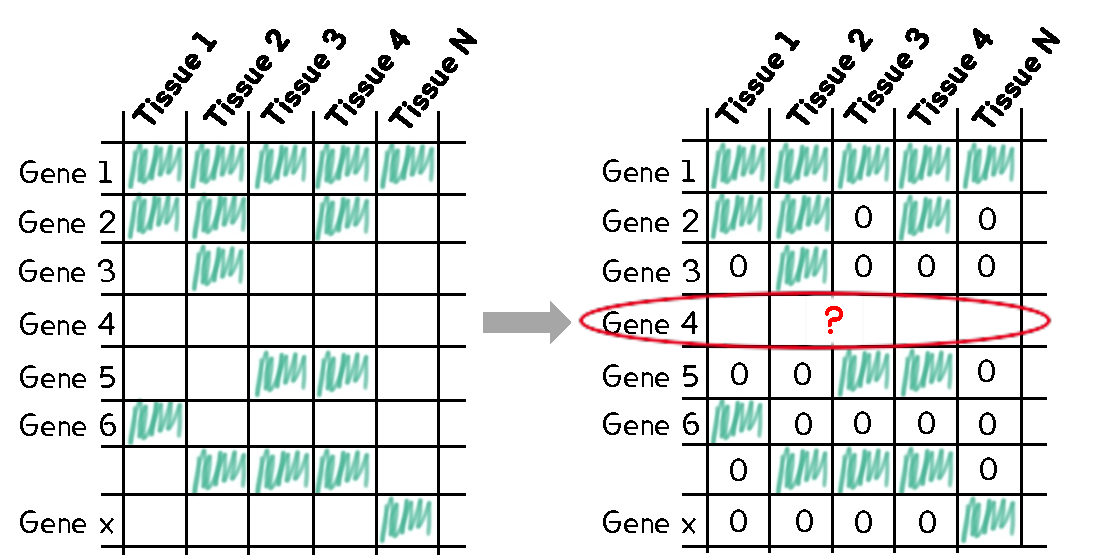
\includegraphics[scale=0.8]{integration/expressedNotExp.pdf}\centering
      \caption[Expressed or not: several cases illustrated]
      {\label{fig:DefineExpression}\textbf{Expressed or not: several cases
      illustrated.}\smallbreak{}Genes as \emph{gene 1} are unequivocal: they have been
      detected in all the different tissues. Genes that have been quantified in
      \emph{some} of the conditions are, in principal, detectable with the
      protocol of sampling and quantification used for the assay.
      For these genes, when no signal is collected, I assume this is a true $0$.
      The genes without any quantification
      in any tissue, e.g.\ gene 4, are discarded from the remaining analysis as
      I can't state
      either there are truly absent from the biological sample or it has to due
      to the protocol at use; they are \emph{undefined}.}
\end{figure}

\subsection{The undefined}\KOMAoptions{parskip=false}
\label{subsec:IntegrationExpressedOrNot-undefined}
If a transcript is never found in any of the samples of a dataset,
then I considered that we can not determine if the transcript was
either truly not expressed or, for any reason, was not captured while the library
preparation or the identification/quantification steps. Hence, those are
excluded from the analyses as I can not resolve precisely if this is a
technical artefact or a biological truth. This case is illustrate by the row
circled in red in~\cref{fig:DefineExpression}.

\subsection{Expression in a dataset}
\label{subsec:IntegrationExpressedOrNot--expDataset}
By contrast, if a transcript is expressed in some samples of the dataset,
then, whenever no expression was recorded in the other
samples, I consider that the expression of the considered macromolecule is truly
null for those samples.

\subsection{Expression within a sample}\KOMAoptions{parskip=half*}\label{subsubsec:exprTrans}
It is a bit more complex as we can expect ``translational noise'' \TKR{}.
While we can empirically evaluate it for each dataset,
there is a widespread (arbitrary) threshold used in the literature:
$1$ \gls{FPKM} (or \gls{RPKM}). In fact,~\citet{Hebenstreit:2011} showed in
their study \paper{\citetitle{Hebenstreit:2011}},
that to be translated into a protein, a \mRNA\ should
present an expression at least equals to $1$ \gls{RPKM}.

As the \Cref{ch:Integration} focuses on the comparison of proteomic and
transcriptomic data, all the analyses have been run with this threshold.
It is worth mentioning that parts of the analyses have also been done without
any threshold or with a threshold of $5$ \glspl{FPKM}.

\subsection*{}

While I have compared the list of undefined, expressed and unexpressed \mRNAs\
through the five datasets,
the bulk of the analysis has been done on the common \mRNAs.

In other words, if a \mRNA\ is not expressed in at least one sample in each
dataset used for the study, it will be excluded from the main part of the
analysis workflow.



\subsection{A consistent pipeline}

\subsection{About correlations}

\subsubsection{Pearson Correlation coefficient}

\section{Results}\label{sec:Trans_Results}
\section{Methods}

%The Pearson product-moment correlation coefficient (often shortened as
%Pearson correlation coefficient or even as correlation coefficient) is a

%
\subsubsection{The expectation}
$E[X]=x_1p_1 + x_2p_2+ \cdots +x_kp_k$

\begin{itemize}
\item $E$ is the expectation
\item $X$ is a random variable
\item $x_1$,$x_2$,\ldots,$x_k$ are possible value of $X$
\end{itemize}




\section{Consistency of processing methodology}\label{sec:Trans_consistentMethodo}

    \subsection{Reuse of processed data issues}\label{subsec:Trans_reuseOfData}

    \subsection{Genome build and annotation impact}\label{subsec:Trans_AnnotImpact}

RNA-seq is consistent across datasets; samples are more likely to cluster by
biological origins than by studies. (Figure 2)
While Pearson correlations are higher, without any a priori Spearman correlations
allow a better separation of the different tissues in distinct clusters across
datasets.

Many genes have a consistent profile of expression levels through the different
datasets.
To help EBI Expression Atlas has developed a feature that allows the visualisation
of the expression of a gene (or protein) across the different dataset that it
integrates. (Figure 3)

Reuse of data allows the assessment of the biological quality of a sample.
While RNA-seq workflows integrate numerous quality checks for their different steps,
it is not always easy to appraise the original quality of the samples. Comparing
similar conditions from different sources allow some high level biological check.
Indeed, we noticed that some tissues have a more unique profile in specific
datasets.

Overall gene expressions for protein coding genes across different tissues
correlated highly between datasets. (See part 3. Integration of Transcriptomics
and Proteomics studies – Figure 15)



    \subsection{Reproducibility of expression profile at tissue level}\label{subsec:Trans_ReproExpresTissue}

        \subsubsection{Correlation}\label{subsubsec:Trans_Tissue_Corr}
        \subsubsection{Clustering}\label{subsubsec:Trans_Tissue_cluster}

    \subsection{Reproducibility of expression profile at gene level}\label{subsec:Trans_ReproExpresGene}

    \subsection{Tissue specific,housekeeping genes and other categories}\label{subsec:Trans_TissueSpeAndHK}

    \subsection{Curated sets}\label{subsec:Trans_curatedSets}

\section{Discussion}\label{sec:Trans_discussion}



\begin{comment}
  \begin{figure}%[!htbp]
      \includegraphics%[scale=0.6]%
      {transcriptomics/}\centering
      \caption[]
      {\label{fig:}\textbf{}}
  \end{figure}
\end{comment}
